\documentclass[tikz,border=8pt]{standalone}
\usepackage{amsmath}
\usetikzlibrary{arrows.meta,positioning,fit,calc}

\begin{document}
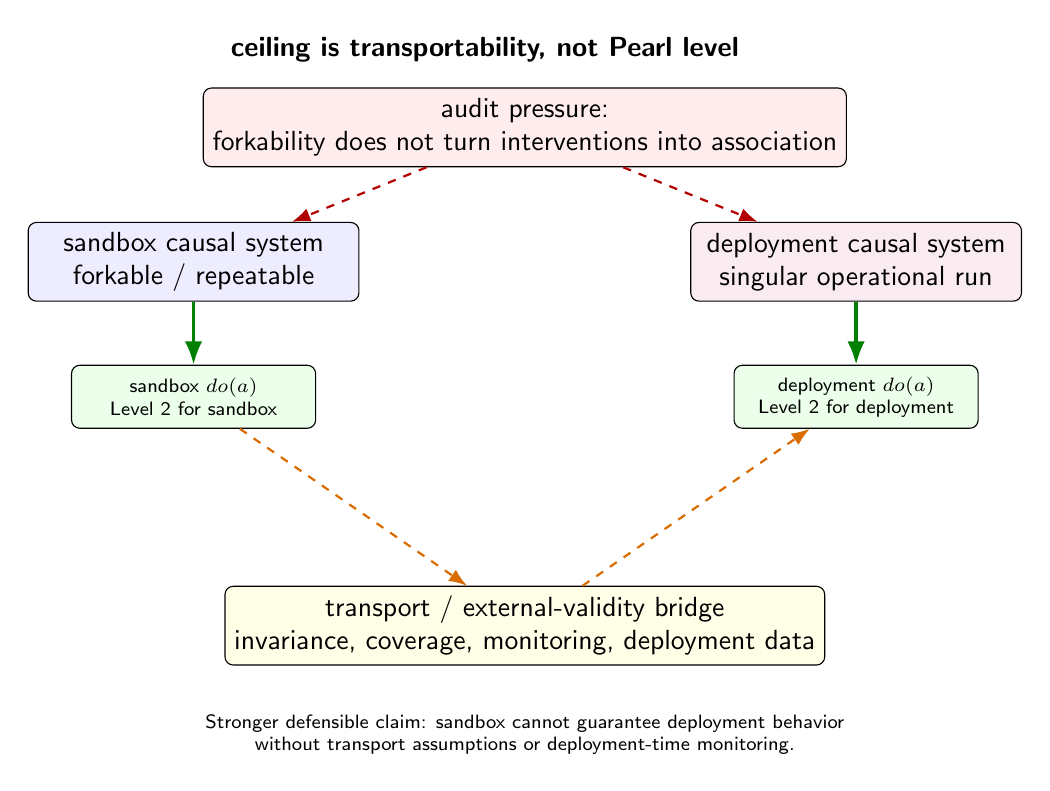
\begin{tikzpicture}[
  font=\sffamily,
  box/.style={draw, rounded corners=3pt, align=center, minimum width=42mm, minimum height=10mm, fill=white},
  small/.style={draw, rounded corners=3pt, align=center, minimum width=31mm, minimum height=8mm, fill=white, font=\sffamily\scriptsize},
  arrow/.style={-Latex, thick, draw=black!65},
  good/.style={-Latex, very thick, draw=green!50!black},
  warn/.style={-Latex, thick, dashed, draw=orange!85!black},
  bad/.style={-Latex, thick, dashed, draw=red!70!black},
  note/.style={align=center, font=\sffamily\scriptsize}
]

\node[font=\sffamily\bfseries] at (3.7,2.7) {ceiling is transportability, not Pearl level};

\node[box, fill=blue!7] (sandbox) {sandbox causal system\\forkable / repeatable};
\node[small, below=8mm of sandbox, fill=green!8] (sdo) {sandbox $do(a)$\\Level 2 for sandbox};
\node[box, right=42mm of sandbox, fill=purple!8] (deploy) {deployment causal system\\singular operational run};
\node[small, below=8mm of deploy, fill=green!8] (ddo) {deployment $do(a)$\\Level 2 for deployment};

\draw[good] (sandbox) -- (sdo);
\draw[good] (deploy) -- (ddo);

\node[box, below=24mm of $(sdo)!0.5!(ddo)$, fill=yellow!10, minimum width=66mm] (transport)
  {transport / external-validity bridge\\invariance, coverage, monitoring, deployment data};
\draw[warn] (sdo) -- (transport);
\draw[warn] (transport) -- (ddo);

\node[box, above=12mm of $(sandbox)!0.5!(deploy)$, fill=red!7, minimum width=70mm] (wrong)
  {audit pressure:\\forkability does not turn interventions into association};
\draw[bad] (wrong) -- (sandbox);
\draw[bad] (wrong) -- (deploy);

\node[note, below=5mm of transport] {
  Stronger defensible claim: sandbox cannot guarantee deployment behavior\\
  without transport assumptions or deployment-time monitoring.
};

\end{tikzpicture}
\end{document}
